\documentclass[tikz,border=10pt]{standalone}
\begin{document}
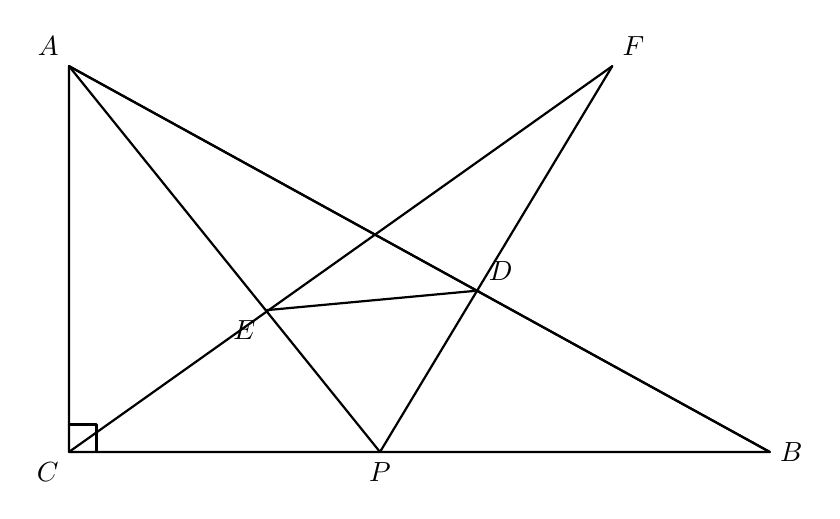
\begin{tikzpicture}[line cap=round, line join=round, thick]
\coordinate (A) at (0,4.9);
\coordinate (B) at (8.9,0);
\coordinate (C) at (0,0);
\coordinate (P) at (3.95,0);
\coordinate (F) at (6.9,4.9);
\coordinate (E) at (2.5,1.8);
\coordinate (D) at (5.2,2.05);

\draw (A) -- (C) -- (B) -- cycle;
\draw (A) -- (B);
\draw (A) -- (P);
\draw (C) -- (F);
\draw (P) -- (F);
\draw (E) -- (D);
\draw (0,0.35) -- (0.35,0.35) -- (0.35,0);

\node[above left] at (A) {$A$};
\node[above right] at (F) {$F$};
\node[right] at (B) {$B$};
\node[below left] at (C) {$C$};
\node[below] at (P) {$P$};
\node[below left] at (E) {$E$};
\node[above right] at (D) {$D$};
\end{tikzpicture}
\end{document}
